\chapter{Asymmetry Detection}

\section{Related Work}
Ferrari \etal~\cite{Ferrari_etal_TMI01} use Gabor filters to estimate the orientation of texture in the image, computing responses at a number of scales, applying PCA somewhere (they don't say why this is sensible), some thresholding (not sure why exactly). They compute a rose diagram (an orientation histogram) ``that represents the difference between the rose diagrams
computed for the left and right mammograms'' and compute three features: entropy (I think they have high/low entropy confused), mean orientation and variance (or dispersion, in which I don't think they account for wraparound). They then classify these 3-vectors using linear discriminant analysis (or ``the Bayesian linear classifier'' as they call it). They reckon that using the mean orientation alone over the whole breast is enough to discriminate between symmetric and asymmetric cases. This is based on a sample of 40 image pairs (20 normal, 20 abnormal). Interestingly, they get sensitivity and specificity values like 77.3\% and 71.4\% and 23.8\% -- with only 40 image pairs, shouldn't these numbers all be to the nearest 2.5\%? It's also difficult to accept that a single architectural distortion in one breast is sufficient to generate a significant difference in global statistics over the whole breast -- on a local level, however, I can believe it.


\subsection{Registration}
In order to compute breast asymmetry, it is sensible to first align the two images:

\begin{itemize}
\item \textbf{Between-side:} This is the easiest case and there must be several examples.
\item \textbf{Between-view:} This is a more interesting but much more difficult scenario where we associate every point in the CC view with a line in the MLO view (or vice versa)~\cite{Kita_etal_CVPR98,vanEngeland_Karssemeijer_IWDM06}
\item \textbf{Between-patient:} For the same view, I suspect this falls in between the previous two scenarios in terms of difficulty. It is, however, difficult to see why you would want to do this.
\end{itemize}

van Engeland and Karssmeijer~\cite{vanEngeland_etal_TMI03} present a comparison of four registration tehcniques: nipple alignment; centre of mass alignment; mutual information-based alignment; and nonrigid image warping (via a thin plate spline). They conclude that nonrigid warping is rubbish, nipple alignment isn't great and the other two are about the same. Correctly segmenting the pectoral muscle and background was found to have a significant effect in several cases.

Kita \etal~\cite{Kita_etal_CVPR98} attempt the difficult between-view case by building a 3D model of the breast from the two projected outlines and applying a model of how the breast might deform under compression. van Engeland and Karssemeijer~\cite{vanEngeland_Karssemeijer_IWDM06} do something similar though I'd need to check details.

Lau and Bischof~\cite{Lau_Bischof_CBR91} is an old paper that aligns the breast via an affine transform computed from three control points estimated from the boundary. They then compute a brightness measure and a roughness measure at each pixel. Combining these (along with their ratio) and a measure of directionality to suppress responses near highly oriented structures (\eg~vessels) they estimate an map of asymmetry between the two breasts.

Wirth \etal~\cite{Wirth_etal_IPA99} use Radial Basis Function as a nonlinear interpolant to achieve nonrigid warping of one breast onto another.

Tahmoush and Samet~\cite{Tahmoush_Samet_SPIE06} locate suspicious points via an interest point detector. What they do then is anyone's guess -- something about a `separator' (classifier?) that uses the difference in distribution of suspicious points between the contralateral breasts to diagnose cancer. I kind of understand what they mean but they are far too vague on details. They proceed to publish an almost identical study (and I mean ``identical'' in the word-for-word sense) in IWDM~\cite{Tahmoush_etal_IWDM06}.

Yin \etal~\cite{Yin_etal_JDI94} use a registration technique described elsewhere before computing something akin to the difference image. They then process this image to look for localized masses.

Miller and Astley~\cite{Miller_Astley_BMVC93} suggest ignoring registration for global asymmetry detection and instead focussing on segmentation such that measures are computed only for regions of the same type of breast tissue. This seems a very sensible approach for global measures at least.


\subsection{Histograms}
Rangayyan \etal~\cite{Rangayyan_etal_JEI07} is probably the closest we'll get to something beyond the usual register-subtract approach. They compute line orientations using Gabor filters and compare, in addition to Hu moments, the statistics of histograms over line orientations between left and right breasts. They use a linear or quadratic classifier to discriminate between healthy and abnormal cases based on subsets of these features, achieving best accuracy with a quadratic classifier and four features (none of which are the Hu moments).

A key question that often arises is that of which histogram distance measure is best. The Earth Mover's Distance (EMD), derived from the \emph{transportation problem}, is often used as one of the better ones for reasons described in Rubner \etal~\cite{Rubner_etal_IJCV00} (which also contains descriptions of some other measures). One problem with the EMD is that it requires iterative optimization to compute which makes it considerably slower than most other metrics. A fast approximation was proposed by Indyk and Thaper~\cite{Indyk_Thaper_SCTV03} and subsequently used for matching contours~\cite{Grauman_Darrell_CVPR04}. A comprehensive list of many distance measures (many of which can be shown to be equivalent) is given by Cha~\cite{Cha_IJMMMAS07}.

Many papers try to model the distribution of a histogram in a Euclidean space, often with a Gaussian distribution (\eg~\cite{Broadhurst_etal_DSSCV05}). This is wrong (and~\cite{Broadhurst_etal_DSSCV05} admit so) whereas other papers look at the problem from a statistical point of view to model the likelihood properly~\cite{Vermeesch_JGR05}. Modelling the distribution of a set of histograms is apparently discussed by Weltje~\cite{Weltje_ESR02} but it's long and I haven't read it yet.

Two more papers may be worth considering. Kadir and Brady~\cite{Kadir_Brady_TR05} present a method for estimating histograms that is less sensitive to quantizing effects; it works by interpolating the sampled signal and computing the histogram of the resulting continuous function. This is more stable than simply histogramming the sampled points, though I suspect it is less accurate in certain circumstances (\ie~a bias-variance tradeoff). Finally, Aherne \etal discuss the merits of the Bhattacharyya distance as the optimal histogram measure~\cite{Aherne_etal_Kybernetika97} (this paper was pointed out to me by Neil Thacker).


\section{Vector Quantization}
One method for determining the similarity of left and right breasts reduces each image to a feature vector with an associated distance measure. In this experiment, we select random patches from normal mammograms, and compute a spatially varying histogram over orientation for each point.

\begin{figure}[t]
	\centering
		\def\figpath{\figroot/asymmetry}
		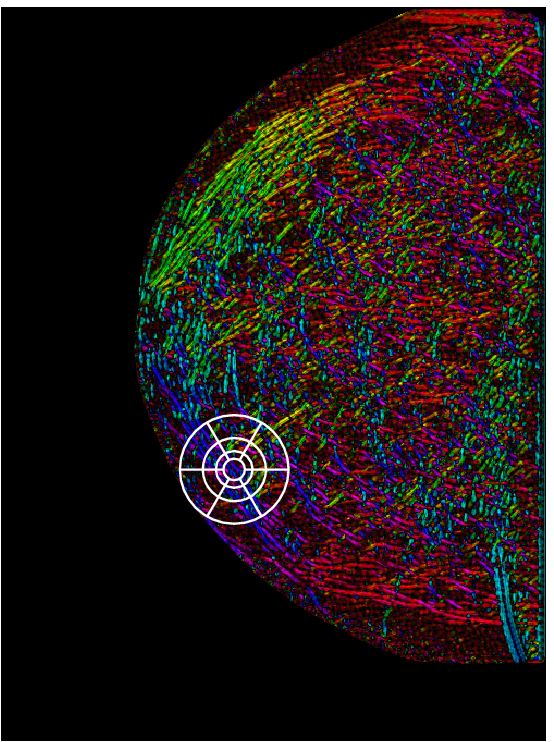
\includegraphics[height=0.3\textheight]{\figpath/roi_full}
		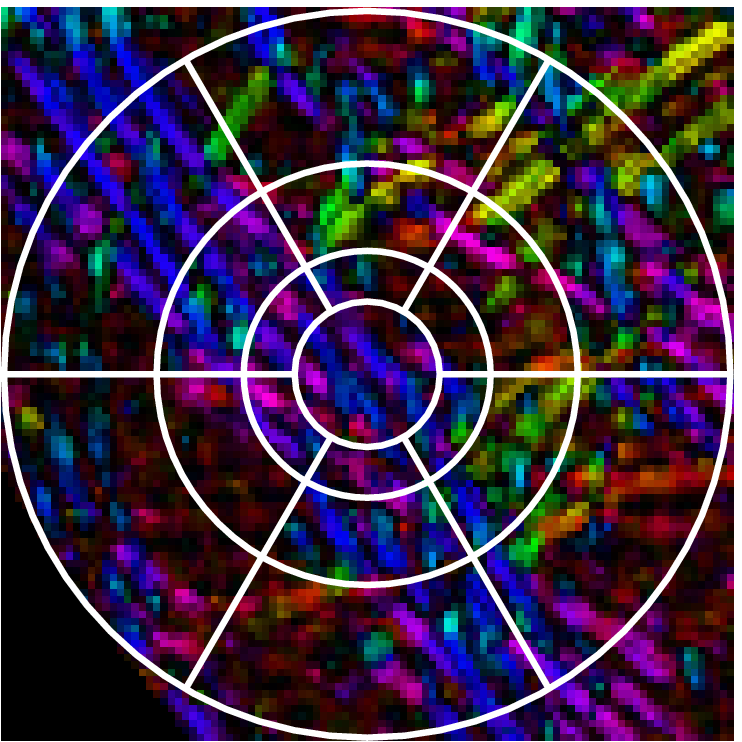
\includegraphics[height=0.3\textheight]{\figpath/roi_zoom}
%
	\caption{Region of Interest overlaid on full image and a close-up.}
	\label{f:logpolar_roi}
\end{figure}

More specifically, we define a log-polar region of interest (\ie~divided linearly by angle and logarithmically by radius) that divides the region into a number of cells (\fref{f:logpolar_roi}). We compute the histogram over orientation for all pixels contained in each cell and concatenate into a single feature vector that captures not only the distribution of orienation within the region of interest but also how it varies spatially (similar to the \emph{f2} feature in Karssemeijer's method~\cite{Karssemeijer_teBrake_TMI96}).

\begin{figure}[t]
	\centering
		\def\figpath{\figroot/asymmetry/centre_001}
		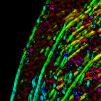
\includegraphics[width=0.15\columnwidth]{\figpath/sample_001}
		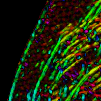
\includegraphics[width=0.15\columnwidth]{\figpath/sample_002}
		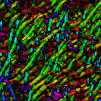
\includegraphics[width=0.15\columnwidth]{\figpath/sample_003}
		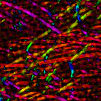
\includegraphics[width=0.15\columnwidth]{\figpath/sample_004}
		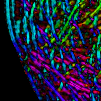
\includegraphics[width=0.15\columnwidth]{\figpath/sample_005}
		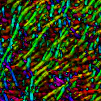
\includegraphics[width=0.15\columnwidth]{\figpath/sample_006}%
		\vspace{2pt}%
		\def\figpath{\figroot/asymmetry/centre_031}
		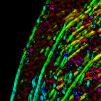
\includegraphics[width=0.15\columnwidth]{\figpath/sample_001}
		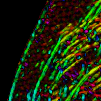
\includegraphics[width=0.15\columnwidth]{\figpath/sample_002}
		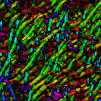
\includegraphics[width=0.15\columnwidth]{\figpath/sample_003}
		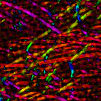
\includegraphics[width=0.15\columnwidth]{\figpath/sample_004}
		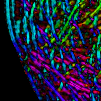
\includegraphics[width=0.15\columnwidth]{\figpath/sample_005}
		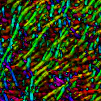
\includegraphics[width=0.15\columnwidth]{\figpath/sample_006}%
		\vspace{2pt}%
		\def\figpath{\figroot/asymmetry/centre_047}
		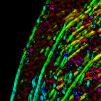
\includegraphics[width=0.15\columnwidth]{\figpath/sample_001}
		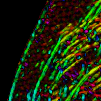
\includegraphics[width=0.15\columnwidth]{\figpath/sample_002}
		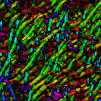
\includegraphics[width=0.15\columnwidth]{\figpath/sample_003}
		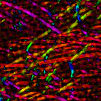
\includegraphics[width=0.15\columnwidth]{\figpath/sample_004}
		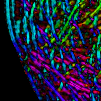
\includegraphics[width=0.15\columnwidth]{\figpath/sample_005}
		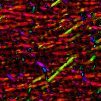
\includegraphics[width=0.15\columnwidth]{\figpath/sample_009}%
		\vspace{2pt}
		\def\figpath{\figroot/asymmetry/centre_046}
		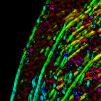
\includegraphics[width=0.15\columnwidth]{\figpath/sample_001}
		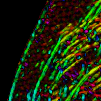
\includegraphics[width=0.15\columnwidth]{\figpath/sample_002}
		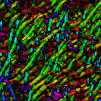
\includegraphics[width=0.15\columnwidth]{\figpath/sample_003}
		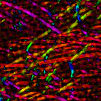
\includegraphics[width=0.15\columnwidth]{\figpath/sample_004}
		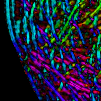
\includegraphics[width=0.15\columnwidth]{\figpath/sample_005}
		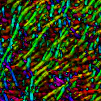
\includegraphics[width=0.15\columnwidth]{\figpath/sample_006}
%
	\caption{Image patches corresponding to four different histogram vector quantization codebook entries.}
	\label{f:codebook_patches}
\end{figure}

Given a set of sampled histograms from normal mammograms, we then cluster the histograms (via K-means) to generate a `codebook' of orientation patterns. Each codebook vector should represent a local orientation pattern in the image (\fref{f:codebook_patches}).

A new image can then be reduced to a feature vector by selecting points at random, computing their orientation histograms, assigning each to a cluster centre, and computing the histogram over cluster assignments. The intuition is that symmetric breasts will exhibit a similar distribution over orientation patterns, such that the distances between the left and right histograms will be, on average, lower in normal (\ie~symmetric) cases than in abnormal (asymmetric) ones.

\begin{figure}[t]
	\centering
		\def\figpath{\figroot/asymmetry}
		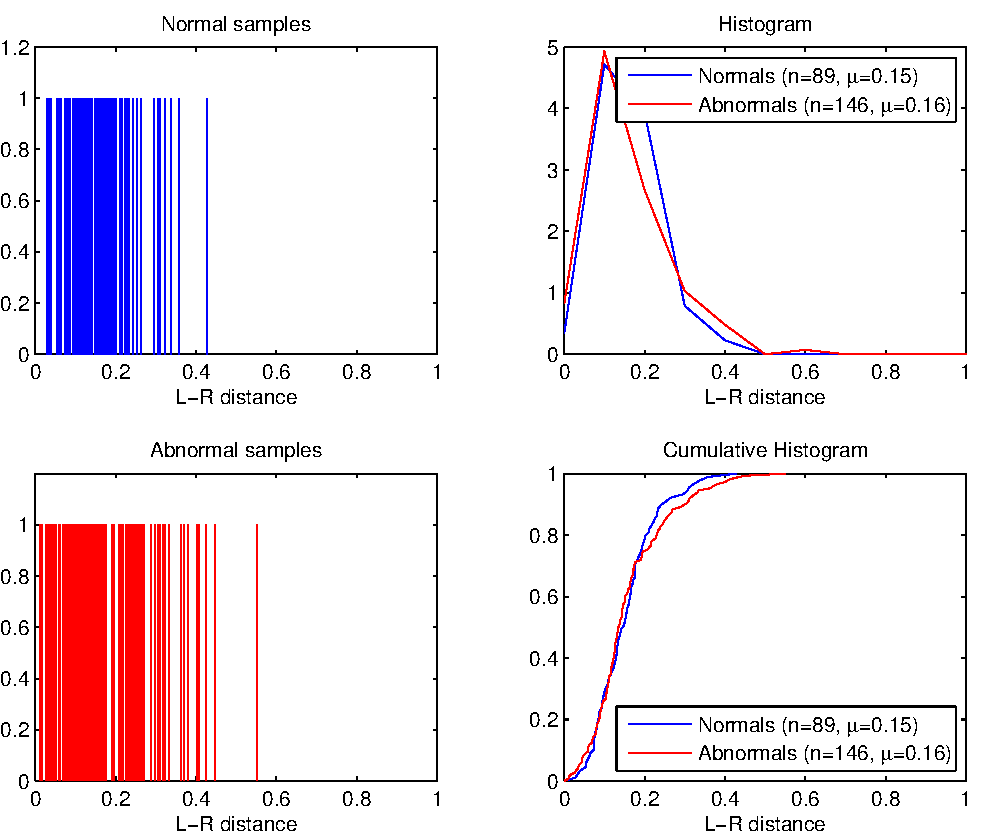
\includegraphics[width = 0.9\columnwidth]{\figpath/graphs}
%
	\caption{Distributions of left-right distance measure for normal and abnormal pairs, viewed as individual samples, a histogram, and a cumulative histogram.}
	\label{f:vq_distances}
\end{figure}

To test the intuition, we computed the left-right distance for all normal pairs (neither of which was used to generate the codebook) and all abnormal pairs. We see a small difference in distribution between normal and abnormal groups, but not enough to build a classifier on (\fref{f:vq_distances}).


\section{Direct Matching}
In another experiment, we looked at matching individual regions of the two images based on a histogram distance between reference and target points. I didn't figure out where to take it from there -- maybe a total distance between left and right, possibly with a Markov Random Field prior to encourage comparison between points that are qualitatively in the same place (\fref{f:hist_matches}).

\begin{figure}[t]
	\centering
	\def\figpath{\figroot/asymmetry}
	\begin{tabular}{c c}
	\begin{minipage}[c]{0.5\columnwidth} 
		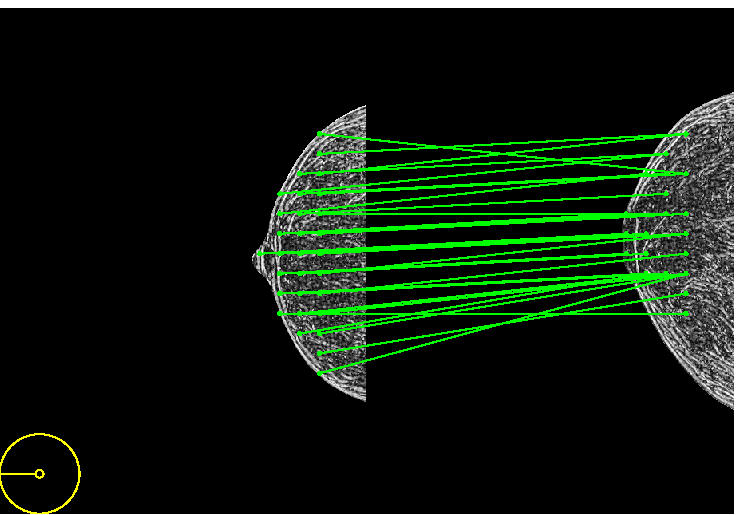
\includegraphics[width=\columnwidth]{\figpath/044LCC_match_matches} 
	\end{minipage}
	\begin{minipage}[c]{0.5\columnwidth}
		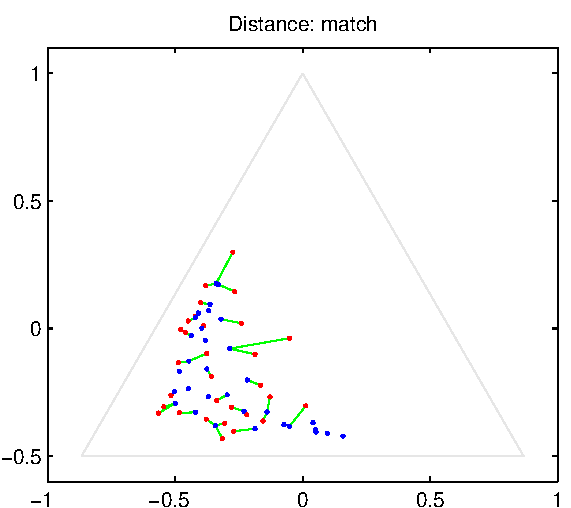
\includegraphics[width=\columnwidth]{\figpath/044LCC_match_hist3d}
	\end{minipage}
	\end{tabular} 
%
	\caption{(left) Matched points on left and right breast images for 044CC; (right) visualization of histograms as points in a plane with matched histograms linked by a line.}
	\label{f:hist_matches}
\end{figure}
